\chapter{Optimized Scheduling}
\label{chap:mode_mapping}

%%%%%%%%%%%%%%%%%%%%%%%%%%%%%%%%%%%%%
%%%%%%%%%%%%%%%%%%%%%%%%%%%%%%%%%%%%%
%%%%%%%%%%%%   SECTION   %%%%%%%%%%%%
%%%%%%%%%%%%%%%%%%%%%%%%%%%%%%%%%%%%%
%%%%%%%%%%%%%%%%%%%%%%%%%%%%%%%%%%%%%
\section{Scheme 3}
\label{sec:mm:scheme4}
According to the A/A Mode processing chain, only Correlation Processing is dependent on the results of the 8 bursts of a dwell. The burst processing chain except the correlation processing has no dependency and can therefor performed independently. The previous 7 bursts. Rest of the processing steps do not have any dependency, thus can be performed independently. The final Correlation Processing shall be computed serially. Space Partition configuration is adopted for Scheme-3 implementation.

\subsection{Hypothesis}
\textbf{\textsl{A Burst shall be processed as soon as a core receives it. This avoids unnecessary waiting time to receive a complete Dwell (8 Bursts) data.}}\\[0.2cm]
In case of the baseline analysis, as illustrated in Figure \ref{fig:mm:scheme4_data_distribution}, beam-forming of the first burst will start only after receiving a complete dwell. Though the first burst is ready for Beam-forming, redundant time is spent in waiting for the complete dwell data. This applies to the Pulse Compression, FFT, and CFAR processing also.

Scheme-3 exploits the fact that every burst can be processed independently until the Thresholding and Detection stage. Every burst is sent to an individual core to process them conveniently as soon as they are received. This saves waiting time during Data receive period, Beam-forming, Pulse compression, FFT and CFAR processing. Nothing has changed in terms of Correlation Processing, hence it will not contribute to the latency reduction.

\subsection{Data distribution}
As shown in Figure \ref{fig:mm:scheme4_aa_mode_mapping}, CPU1...6 are allocated for burst processing and CPU7 executes four instances of Correlation Processing in four cores, performing one instance per core. Burst processing comprises of Beam-forming, Pulse Compression, FFT and CFAR processing. A burst processing CPU gets four bursts and executes one instance of burst processing per core.

\begin{tabular}{rl}
	No.of cores for burst processing: & 6 x 4 = 24 \\
	No.of cores for correlation processing: & 1 x 4 = 4 \\
	Data distribution-burst processing: & One burst per core \\
	Data distribution-correlation processing: & One dwell per core \\
\end{tabular}
%\FloatBarrier 

\begin{figure}[h!]
	\centering
	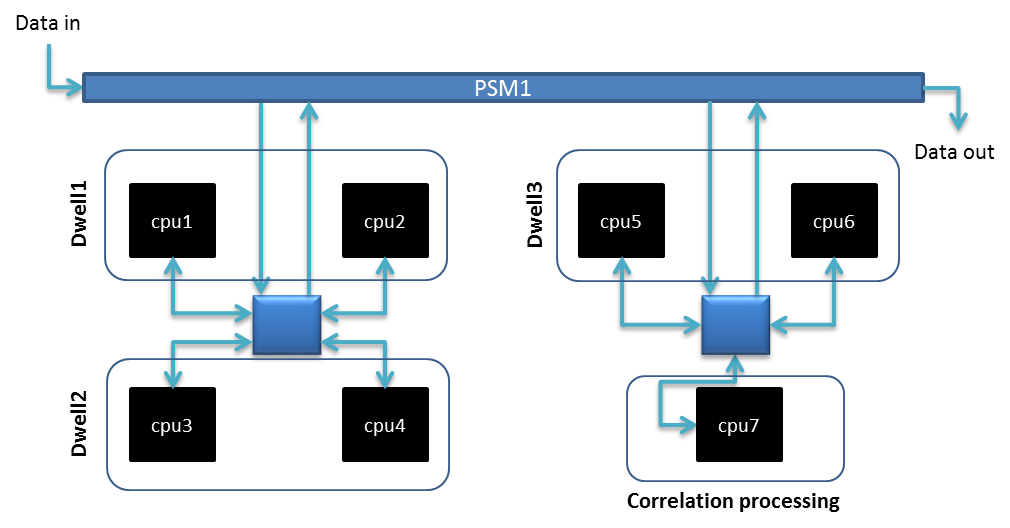
\includegraphics[width=140mm]{figures/scheme4_aa_mode_mapping}
	\caption{Scheme-3, Mode Mapping}
	\label{fig:mm:scheme4_aa_mode_mapping}
\end{figure}

\vspace*{0.2cm}
\noindent
The received A/A mode raw data will be processed as follows

\begin{enumerate}
\item PSM1 routes each burst data to each core starting from core1 of CPU1 to core4 of CPU6 in round robin fashion.
\item Each core in the CPU1...6 performs burst processing followed by storing the results in SDRAM.
\item In a burst processing CPU, a core completing the processing steps last will transfer all the cores(core1...4) results to the CPU7 for correlation processing. This avoids frequent communication between burst processing CPUs and correlation processing CPU. The data passed to the CPU7 is alarm list and their related information, which is smaller in size and assumed that it requires only 0.01ms to transfer.
\item Each core of the CPU7 waits for processed 8 burst data, and then performs Correlation Processing followed by sending out the target detections to PSM1.
\item PSM1 directs the results to tracking processor or display processor. Data distribution scheme is shown in Figure \ref{fig:mm:scheme4_data_distribution}.
\end{enumerate}

\begin{figure}[h!]
	\centering
	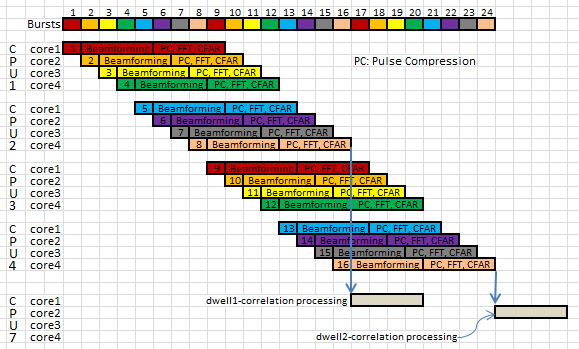
\includegraphics[width=140mm]{figures/scheme4_data_distribution.png}
	\caption{Scheme-3, Data Distribution}
	\label{fig:mm:scheme4_data_distribution}
\end{figure}

\begin{figure}[h!]
	\centering
	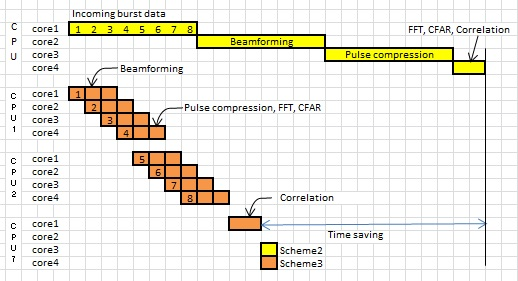
\includegraphics[]{figures/scheme4_comparison}
	\caption{Comparison of Data Distribution Schemes}
	\label{fig:mm:scheme4_comparison}
\end{figure}

Another difference between Scheme-1 and Scheme-3 is the amount of data processed by a CPU. Scheme-1 performs 8 bursts processing whereas Scheme-3 performs 4 bursts processing per CPU. This decreases memory requirement and memory transfer bandwidth compared to the Scheme-1.

\subsection{Processing Latency}
\label{ss:mm:scheme4:latency}
Processing latency is measured on a real hardware clocked 1GHz and the results are scaled down to 800MHz. Data transfer time of 0.02ms is assumed between CPU1...6 and CPU7. Total time required to process one burst until Thresholding and Detection stage is same as Scheme-1, the differences here are 

\begin{compactitem}
	\item Four bursts are distributed to a CPU.
	\item OS overhead factor is removed.
	\item Data copy times among the cores are ignored, as the Time Domain Processing, Frequency Domain Processing and Detection Processing of a burst are performed in individual cores.
	\item The \textsl{Sum of required time} values in Figure \ref{fig:mm:scheme4_elapsed_time} are different from Scheme-1 because the execution cycle of the benchmarks are evaluated and updated (see Chapter \ref{mm:cons:exe_cyl_mismatch}).
\end{compactitem}
\vspace*{0.2cm}
Processing latency calculations are same as explained in Chapter \ref{sss:scheme1:aa:cpu_util}. Details of the look direction2,3,4 are not shown for simplicity.
\begin{figure}[h!]
	\centering
	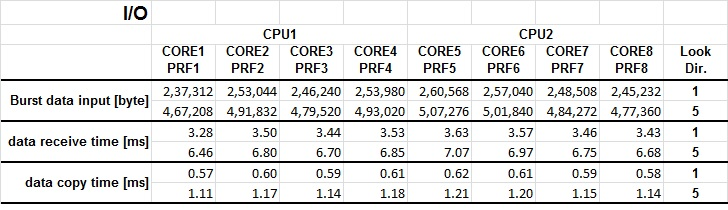
\includegraphics[width=140mm]{figures/scheme4_io}
	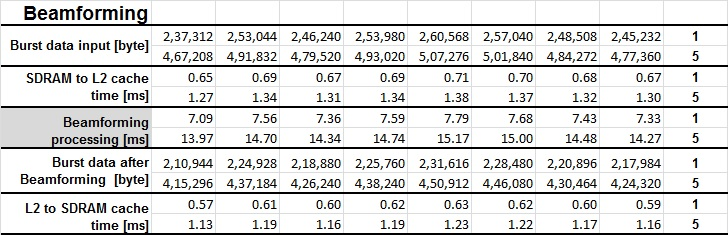
\includegraphics[width=140mm]{figures/scheme4_bf}
	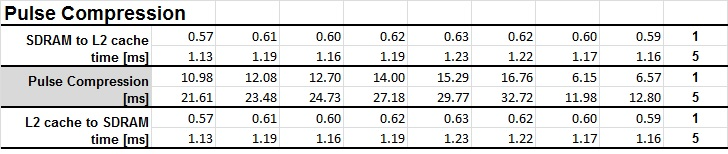
\includegraphics[width=140mm]{figures/scheme4_pc}
	\caption{Scheme-3, Input Output, Beamforming and Pulse Compression}
	\label{fig:mm:scheme4_io}
\end{figure}

The stated values in Figure \ref{fig:mm:scheme4_fft} say that the look direction-1, PRF1 needs 35.72ms time to complete the execution from the moment a core starts receiving a burst. Elapsed wall clock time to process burst by burst is listed as \textsl{Time spent} in the Figure \ref{fig:mm:scheme4_elapsed_time}. Example calculations for the look direction-1 are explained here with reference to the Figure \ref{fig:mm:scheme4_timeline_burst_proc}. A core waits for the pre-defined burst data to be received, i.e. a core processing PRF5 should wait till the PRF1...5 are distributed by the iCON. Burst receive time are derived from the Radar characteristics (see Chapter \ref{ss:aa_mode:radar_char}). PRF7 requires lesser time to process a burst than PRF6, because N$_{rg}$=59 for PRF7, requires 64-point(next power of 2) convolution, on the other hand N$_{rg}$=68 for PRF6, requires 128-point convolution.

\begin{figure}[h!]
	\centering
	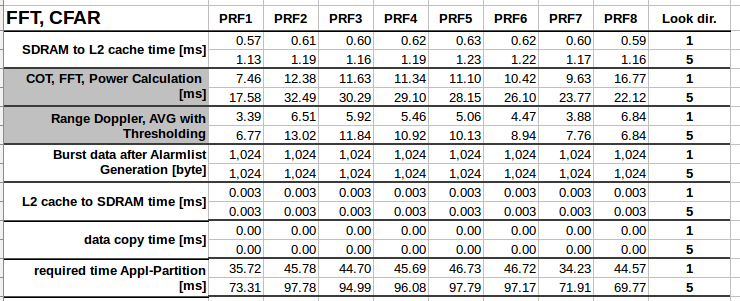
\includegraphics[width=140mm]{figures/scheme4_fft}
	\caption{Scheme-3, FFT and CFAR Processing}
	\label{fig:mm:scheme4_fft}
\end{figure}

\begin{figure}[h!]
	\centering
	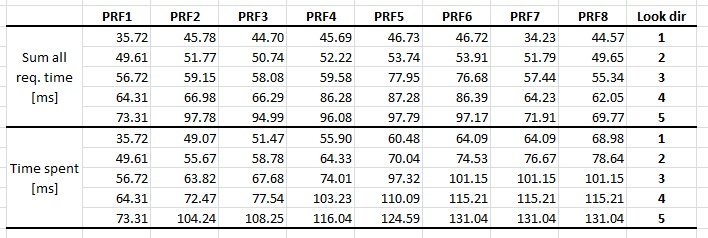
\includegraphics[width=140mm]{figures/scheme4_elapsed_time}
	\caption{Scheme-3, Processing Time}
	\label{fig:mm:scheme4_elapsed_time}
\end{figure}

\begin{align*}
	Elapsed \: time &= MAX((Previous \: burst \: receive \: time + Execution \: time), Elapsed \: time)\\
	PRF1 &= MAX((0 + 35.72), 0) = 35.72 \: ms\\
	PRF2 &= MAX((PRF1 \: receive \: time + Execution \: time), Elapsed \: time) \\
		&= MAX((3.28 + 45.78), 35.72) = 49.07 \: ms \\	 
	PRF3 &= MAX((PRF1...2 \: receive \: time + Execution \: time), Elapsed \: time) \\	
		&= MAX((3.28 + 3.50 + 44.7),49.07) = 51.47 \: ms \\
	PRF4 &= MAX((3.28 + 3.50 + 3.44 + 45.69), 51.47) = 55.90 \: ms \\
	PRF5 &= MAX((3.28 + 3.50 + 3.44 + 3.53 + 46.73), 55.90) = 60.48 \: ms \\
	PRF6 &= MAX((3.28 + 3.50 + 3.44 + 3.53 + 3.63 + 46.72), 60.48) = 64.09 \: ms \\ 
	PRF7 &= MAX((3.28 + 3.50 + 3.44 + 3.53 + 3.63 + 3.57 + 34.23), 64.09) = 64.09 \: ms \\	
	PRF8 &= MAX((3.28 + 3.50 + 3.44 + 3.53 + 3.63 + 3.57 + 3.46 + 44.57), 64.09) \\
		&= 68.98 \: ms	\stepcounter{equation}\tag{\theequation}
\end{align*}

\begin{figure}[h!]
	\centering
	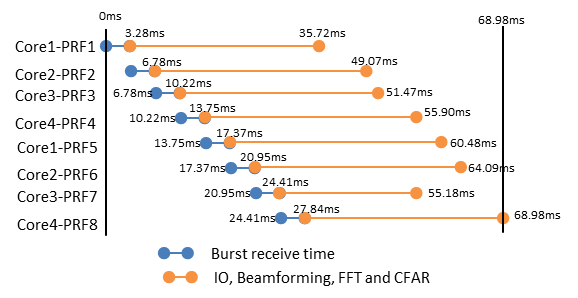
\includegraphics[width=130mm]{figures/scheme4_timeline_burst_proc}
	\caption{Scheme-3, Elapsed Time Calculation}
	\label{fig:mm:scheme4_timeline_burst_proc}
\end{figure}

Data transfer time of 0.02ms between burst processing CPUs and correlation processing CPU, and 0.2ms between correlation processing CPU and tracking/display processor is assumed.
\begin{align*}
	Latency &= Burst \: processing + Data \: transfer \: to \: CPU7 + Correlation \: processing \\
		& \qquad + Transfer \: results  \\
		&= 68.98 + 0.02 + 43.34 + 0.2 = 112.5 \: ms  \stepcounter{equation}\tag{\theequation}
\end{align*}
The processing latency between 112.52ms and 174.58ms are achieved depending on the look direction. Table \ref{tbl:mm:scheme4_latency} lists the processing latency of every look direction.
\begin{table}[h!]
	\centering
	\begin{tabular}{|c|l|l|l|} 
	 \hline
	 \textbf{Look direction} & \textbf{Dwell time[ms]} & \textbf{Latency[ms]} & \textbf{\#Dwell latency} \\
	 \hline
	 1 & 27.84 & 112.52 & 4.04 \\ \hline
	 2 & 33.07 & 122.18 & 3.69 \\ \hline
	 3 & 39.17 & 144.69 & 3.69 \\ \hline
	 4 & 46.20 & 158.75 & 3.44 \\ \hline
	 5 & 54.26 & 174.58 & 3.22 \\ \hline
	\end{tabular}
	\caption{Scheme-3, Processing Latency}
	\label{tbl:mm:scheme4_latency}
\end{table}
\FloatBarrier

\subsection{CPU Load}
\label{ss:mm:scheme4:cpu_load}
CPU load is the ratio of processing time to the available time. 6 CPUs are involved in A/A mode processing; meaning 24 cores are processing 24 burst (3 dwell) data. Available time is 3x dwell time. From the Figure \ref{fig:mm:scheme4_util}, maximum core utilization can reach up to 66\%. Calculations for the look direction-1, PRF1 are explained here.
\begin{figure}[h!]
	\centering
	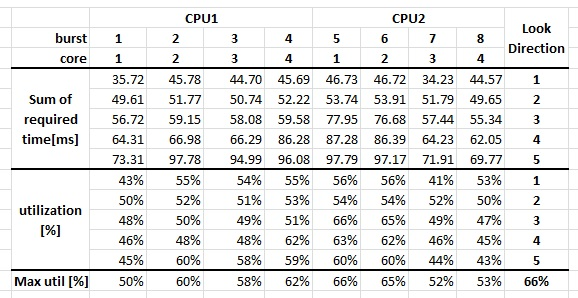
\includegraphics[width=140mm]{figures/scheme4_util}
	\caption{Scheme-3, CPU Utilization}
	\label{fig:mm:scheme4_util}
\end{figure}

\begin{align*}
	Required \: time &= 35.72 \: ms \\
	Available \: time &= 3 * dwell \: time = 3 * 27.84 = 82.2\: ms \\
	Utilization &= \frac{Required \: time}{Available \: time} = \frac{35.72}{82.2} = 43.4\% \stepcounter{equation}\tag{\theequation}
\end{align*}

\clearpage
\subsubsection{Utilization of Correlation Processing CPU}
\label{mm:SSS:scheme4:corr_cpu_util}
Updated correlation processing time values are listed in Figure \ref{fig:mm:scheme4_corr_calc}. The calculations are the same as used in Scheme-1, the difference is that the operating system overhead factor is removed from the analysis.
\begin{figure}[h!]
	\centering
	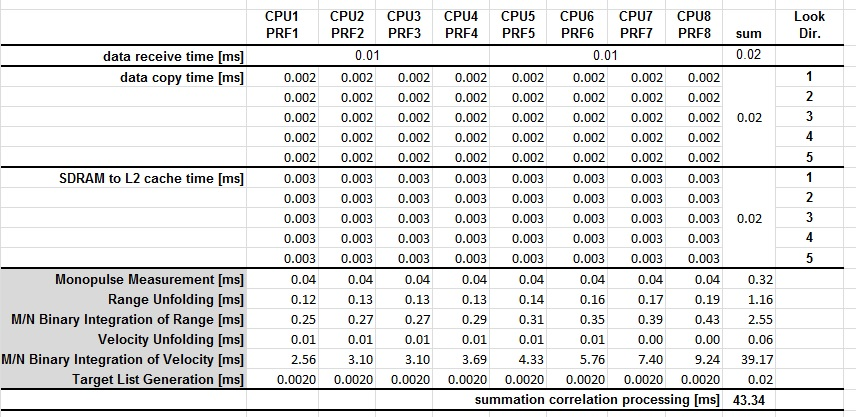
\includegraphics[width=160mm]{figures/scheme4_corr_proc}
	\caption{Scheme-3, Execution Time of Correlation Processing}
	\label{fig:mm:scheme4_corr_calc}
\end{figure}

Every core of the correlation processing CPU is in idle state until it receives results of the 8 burst data from CPU1...6. Then it continues processing for 43.34ms before returning to idle state. Dwells are distributed to 4 cores of the CPU7 in round robin manner. From the Table \ref{tbl:mm:scheme4_corr_cpu_util}, peak utilization of the CPU7 is 39\%. 

Core1 of the CPU7 can start processing as soon as 8 bursts of a dwell are received. 1ms delay is assumed between burst processing CPUs sending out the data and CPU7 starts processing. From the Figure \ref{fig:mm:scheme4_elapsed_time}, look direction-1 needs 68.98ms to do burst processing. Until this time, core1 of the CPU7 is in idle state. Correlation processing takes place for the next 43.34ms in core1 followed by waiting for the next set dwell5 data. Dwell5 will be supplied to the burst processing CPUs at 115.3ms (4 x 27.84ms) by the incoming data stream. Received dwell5 data will be fed to CPU7 after 68.98ms (processing) + 1ms (transfer). Utilization calculation for the look direction-1 is depicted in Figure \ref{fig:mm:scheme4_corr_cpu_util}, and the core1's utilization is derived as follows.

\begin{figure}[h!]
	\centering
	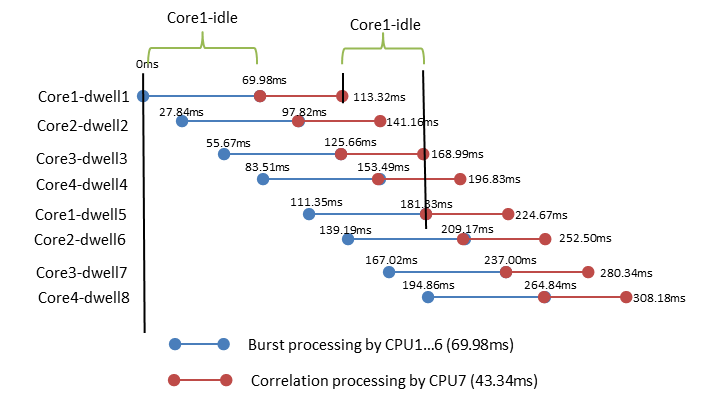
\includegraphics[width=160mm]{figures/scheme4_corr_timeline}
	\caption{Look Direction-1, Utilization of the Correlation Processing CPU}
	\label{fig:mm:scheme4_corr_cpu_util}
\end{figure}

\begin{align*}
	Utilization \: at \: dwell1 &= \frac{processing \: time}{processing \: time + Idle \: time } = \frac{43.34}{43.34 + 69.98} = 38\% \\[0.4cm]
	Next \: dwell \: time &= Dwell5 \: input \: at \: burst \: processing + Burst \: processing \: time \\
	&= 4 * 27.84 + 69.98 =181.3 \: ms\\
	Idle \: time &= Next \: dwell \: in - Last \: dwell \: out \\
	&= 181.33 - (69.98 + 43.34) = 68.01 \: ms \\
	Utilization \: at \: dwell5 &= 	\frac{43.34}{43.34 + 68.01} = 39\%  \stepcounter{equation}\tag{\theequation}
\end{align*}

\begin{table}[h!]
	\centering
	\begin{tabular}{|c|l|} 
	 \hline
	 \textbf{Look direction} & \textbf{Max CPU Utilization} \\
	 \hline
	 1 & 39\%  \\ \hline
	 2 & 35\%  \\ \hline
	 3 & 30\%  \\ \hline
	 4 & 27\%  \\ \hline
	 5 & 25\%  \\ \hline
	\end{tabular}
	\caption{Utilization of Correlation Processing CPU}
	\label{tbl:mm:scheme4_corr_cpu_util}
\end{table}
Utilization drops for ascending look direction, since look direction 5 has longest data receive time and processing time but maximum target detections are same for all the look directions. 

\subsection{Memory Transfer Bandwidth}
\label{ss:mm:scheme4:bw_util}
The lowest recorded memory transfer bandwidth by running the STREAM benchmark as a background task is listed in Table \ref{tbl:mm:scheme4_mem_bw} 
Peak memory transfer bandwidth of the Radar application is measured as 39.4\% of the available 1048MiB/s.

\begin{table}[h!]
	\centering
	\begin{tabular}{|l|l|l|l|l|} 
	 \hline
	 \textbf{Function} & \textbf{Best Rate [MB/s]} & \textbf{Avg time[s]} & \textbf{Min time[s]} & \textbf{Max time[s]} \\
	 \hline
	 Copy & 635.0 &0.264075 & 0.251953 & 0.272976 \\ \hline
	\end{tabular}
	\caption{Recorded Memory Transfer Bandwidth of the STREAM Benchmark Running as Background Task}
	\label{tbl:mm:scheme4_mem_bw}
\end{table}

\begin{align*}
\label{aa:scheme4:mem_bw}
	Peak \: BW \: of \: the \: Radar \: application &= Idle \: BW - Lowest \: recorded \: BW \\
	&= 1048 - 635 = 413 \: MiB/s \\
	&= \frac{413}{1048} = 39.4 \% \stepcounter{equation}\tag{\theequation} 
\end{align*}

\subsection{Memory Utilization}
\label{ss:mm:scheme4:mem_util}
From the \verb|mem_util.sh| script, it is measured that the Radar application is consuming only 0.9\% of the available 879MiB memory. Memory utilization footprint of the Radar application is shown in Figure \ref{fig:mm:scheme4_mem_util}.

\begin{figure}[h!]
	\centering
	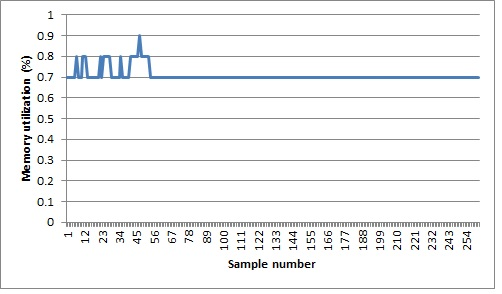
\includegraphics[width=100mm]{figures/scheme4_mem_util}
	\caption{Scheme-3, Memory Utilization Footprint}
	\label{fig:mm:scheme4_mem_util}
\end{figure}

\subsection{Summary}
\label{ss:mm:scheme4:summary}
Scheme-3 has 4x dwell time latency, 66\% CPU utilization, 41\% memory transfer bandwidth utilization and 1\% memory utilization. CPU utilization can be improved by adding more DGPMs. An IMA processor architecture can have upto 6 DGPMs comprising of 24 CPUs. Scheme-3 has utilized 28 cores of 7 CPUs, while rest of the 17 CPUs can be used for other purpose including A/G mode processing. A comparison of Scheme-1, Acceptable values and Scheme-3 is given below.

\begin{table}[h!]
	\centering
	\begin{tabular}{|l|l|l|l|} 
	 \hline
	 \textbf{Parameter} & \textbf{Scheme-1} & \textbf{Acceptable Values} & \textbf{Scheme-3}\\
	 \hline
	 Dwell latency &  14.96 & 2 & 4.04 \\ \hline
	 CPU load & 75.5\% & \textless 50\% & 66\% \\ \hline
	 Memory utilization & 7\% & \textless 50\%  & 1\% \\ \hline
	 Memory transfer bandwidth & NA & \textless 50\% & 41\%  \\ \hline
	\end{tabular}
	\caption{Comparison of Scheme-1 vs Acceptable Values vs Scheme-3}
	\label{tbl:mm:scheme4_comparison}
\end{table}

\clearpage
%%%%%%%%%%%%%%%%%%%%%%%%%%%%%%%%%%%%%
%%%%%%%%%%%%%%%%%%%%%%%%%%%%%%%%%%%%%
%%%%%%%%%%%%   SECTION   %%%%%%%%%%%%
%%%%%%%%%%%%%%%%%%%%%%%%%%%%%%%%%%%%%
%%%%%%%%%%%%%%%%%%%%%%%%%%%%%%%%%%%%%
\section{Scheme 4}
\label{sec:mm:scheme5}
Space Partition configuration is adopted for Scheme-4 implementation.
\subsection{Hypothesis}
\begin{compactitem}

\item Taking a closer look into the processing chain in Chapter \ref{sec:bg_related_work:proc_chain}, revels that a burst data has 4 channel processing namely Sum, Guard, Azimuth and Elevation.  These 4 channels do not have data dependency, allowing for parallel execution. Figure \ref{fig:mm:scheme5_data_path}, shows the data dependency diagram for A/A mode processing.

\begin{figure}[h!]
	\centering
	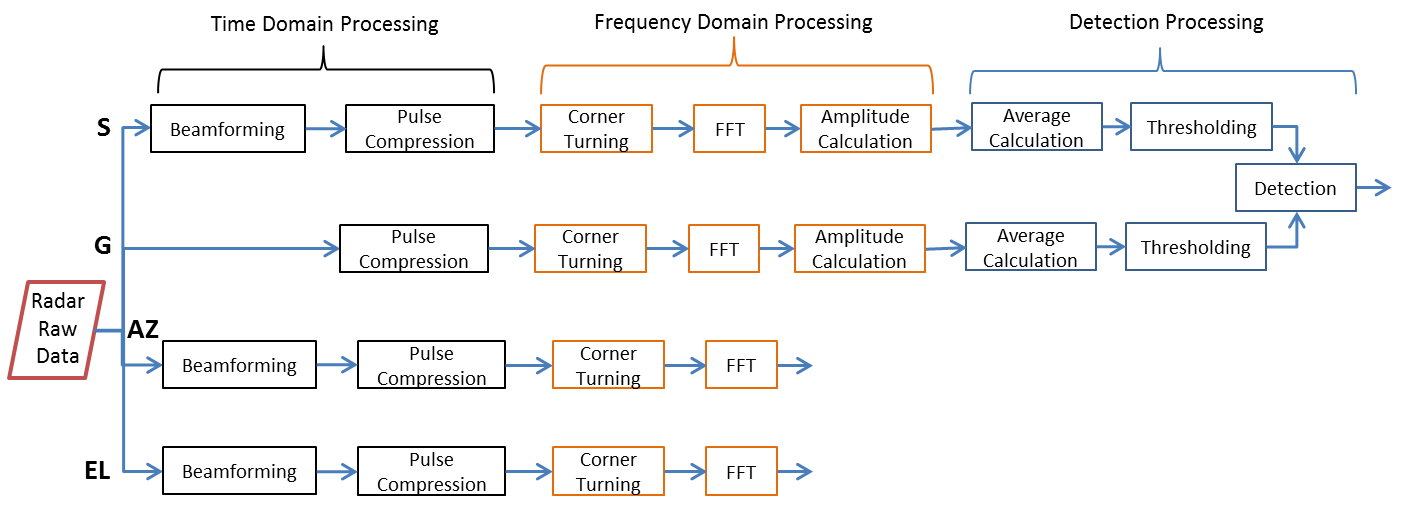
\includegraphics[width=160mm]{figures/scheme5_data_path}
	\caption{A/A Mode - Data Dependency of the Radar Application}
	\label{fig:mm:scheme5_data_path}
\end{figure}
Note: The data dependency diagram doesn't consider constant table values such as Sum channel beamforming vector, Azimuth channel beamforming vector, etc, as they are pre-calculated and available at any point of time.

\item Correlation processing shall be optimized to bring down the execution time.
\end{compactitem}

\subsection{Data Distribution}
\label{ss:mm:scheme5:data_distribution}
Four channel processing are done by 4 cores of a CPU. CPU1...12 gets one burst each. CPU13 and CPU14 are allocated for correlation processing. 
PSM1 routs the Radar raw data to the respective DGPMs. Burst results are sent to PSM1 by the CPUs 1..12. PSM1 stores the burst result until 8 burst results are received. Then 8 burst results are sent to the cores of CPU13 and CPU14 in round robin manner. The DGPMs and PSM are arranged as shown in Figure \ref{fig:mm:scheme5_mode_mapping} and the data distribution is illustrated in Figure \ref{fig:mm:scheme5_data_distri}.

\begin{figure}[h!]
	\centering
	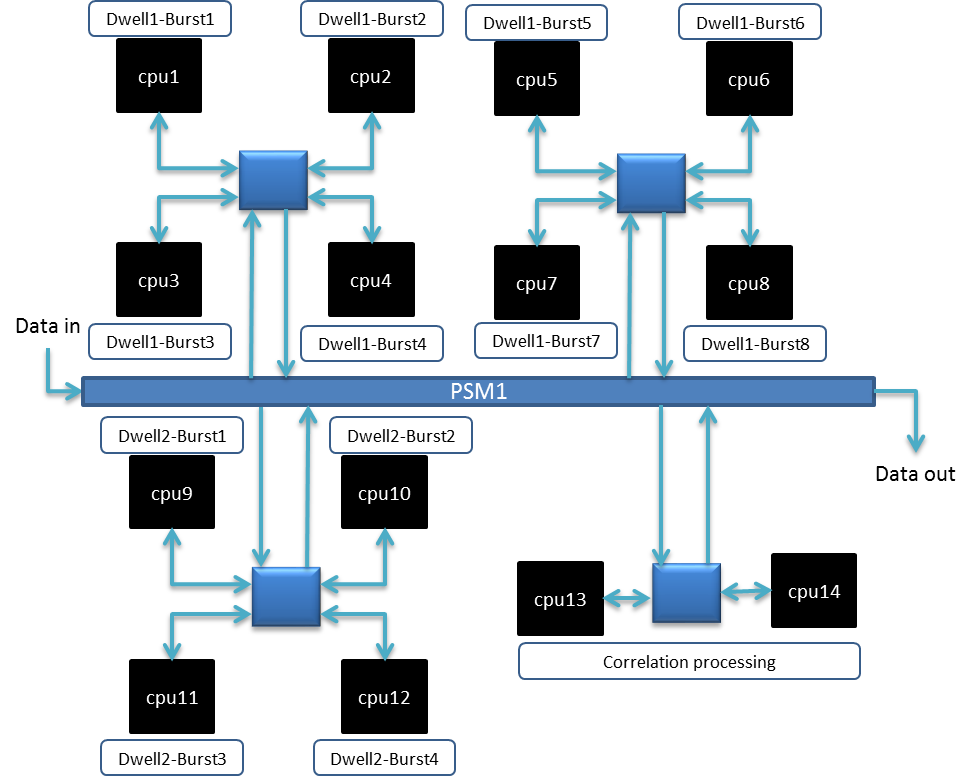
\includegraphics[width=130mm]{figures/scheme5_mode_mapping}
	\caption{Scheme-4, Mode Mapping}
	\label{fig:mm:scheme5_mode_mapping}
\end{figure}

\begin{figure}[h!]
	\centering
	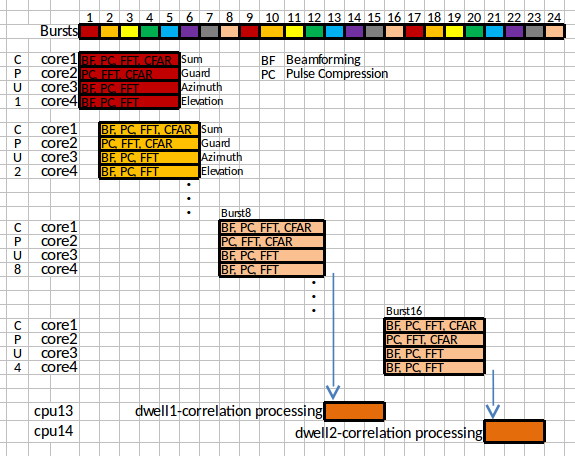
\includegraphics[width=130mm]{figures/scheme5_data_distri}
	\caption{Scheme-4 Data Distribution}
	\label{fig:mm:scheme5_data_distri}
\end{figure}

\begin{figure}[h!]
	\centering
	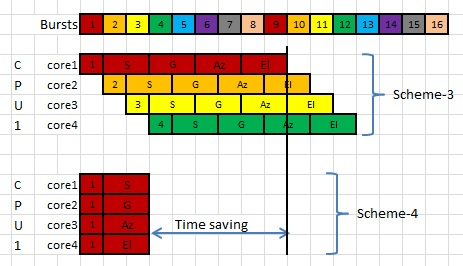
\includegraphics[width=95mm]{figures/scheme5_time_saving}
	\caption{Scheme-3 vs Scheme-4}
	\label{fig:mm:scheme5_time_saving}
\end{figure}

In terms of burst processing, every CPU in Scheme-3 performs computation on 4 burst data, whereas a CPU in Scheme-4 does computations on one burst. Single burst is placed in the shared memory, so that all the four cores can access them. CPU1 gets the first burst. Core1 of the CPU1 performs Beamforming, Pulse Compression, FFT and CFAR processing of Sum channel on the burst data. Rest of the three cores repeat the same for Guard channel, Azimuth and Elevation channel processing simultaneously. It results in approximately 4x reduced memory requirement than Scheme-3. A comparison of Scheme-3 and Scheme-4 is shown in Figure \ref{fig:mm:scheme5_time_saving}.

Correlation processing requires 43.34ms (see Chapter \ref{mm:SSS:scheme4:corr_cpu_util}) to process one dwell data. Dwell time of the look direction-1 is 27.84ms. Correlation processing itself consumes 1.5x dwell time. Best result cannot be achieved without optimizing the correlation processing. According to the derivations of measurement time, M/N Binary Integration of Velocity consumes 39.16ms of total 43.34ms. It is a good candidate for optimization. M/N Binary Integration of Velocity is implemented in \verb|C| program according to the pseudo-code shown in Algorithm \ref{mm:biv:pseudo_code} and the execution time is measured as 31.72ms when four instances are running on four cores. The loop iterations(Line 3) of a single instance of M/N velocity integration are independent of the previous loop processing and next loop processing. They are broken into four loops to run on four cores of a CPU in parallel. 4x speedup is achieved for M/N Binary Integration of Velocity, reducing execution time from 31.72ms to 7.93ms. Any correlation processing CPU in Scheme-4 processes one dwell data, on contrary to the 4 dwell data in Scheme-3. Data distribution scheme and time saving are shown in Figure \ref{fig:mm:scheme5_corr_dd}, data dependency is shown in Figure \ref{fig:mm:scheme5_corr_data_path}. Data structures of the Range Correlation Information(RCI) and Correlation Matrix Velocity(CMV) are depicted in Figure \ref{fig:mm:biv_struct}. These two data structures are the results of previous correlation processing steps namely Monopulse measurement, Range unfolding, M/N range integration and Velocity unfolding.

\renewcommand{\algorithmicrequire}{\textbf{Input:}}
\renewcommand{\algorithmicensure}{\textbf{Output:}}

\begin{algorithm}
\caption{Pseudocode - Binary Integration of Velocity\cite{fcas}.}
\label{mm:biv:pseudo_code}
\begin{algorithmic}[1]
	\Require 
		\Statex \texttt{M$_v$:} Binary integration threshold from constant table
		\Statex \texttt{W$_{size}$:} Velocity window size from constant table
		\Statex \texttt{RCI} and \texttt{CMV} from previous processing steps
	\Ensure
		\Statex Updated \texttt{RCI}
		\Statex

	\LState \texttt{b\_ref = burst\_id;}
	\LState \texttt{n\_rc = RCI.N$_{rc}$}
	\For{\texttt{n:=1 to n\_rc}}
		\LState \texttt{ai\_ref = RCI.RCI\_PREV[n].AI;}
		\LState \texttt{n\_burst = RCI.RCI\_PREV[n].N$_{bc}$;}
		\LState \texttt{best\_count = M$_v$-1;}
		\LState \texttt{best\_v = 0;}
		\LState \texttt{count = 0;}
		
		\For{\texttt{ref\_unf:=1 to CMV.CMV\_PREV[b\_ref].AI[ai\_ref].N$_{unf}$}}
			\LState \texttt{v\_ref = CMV.CMV\_PREV[b\_ref].AI[ai\_ref].V[ref\_unf];}
			
			\For{\texttt{m:=1 to n\_bursts}}
				\LState \texttt{b\_cmp = RCI.RCI\_PREV[n].BI[m].BID;}
				\LState \texttt{ai\_cmp = RCI.RCI\_PREV[n].BI[m].AL;}
				\LState \texttt{cmp\_unf =  CMV.CMV\_PREV[b\_cmp].AI[ai\_cmp].N$_{unf}$;}
				
				\For{\texttt{k:=1 to cmp\_unf}}
					\LState \texttt{v\_cmp = CMV.CMV\_PREV[b\_cmp].AI[ai\_cmp].V[k];}
					\LState \texttt{diff\_v = v\_cmp - v\_ref;}
					
					\If{\texttt{((diff\_v <= W$_{size}$) \&\& (sign(v\_cmp)==sign(v\_ref)))}}
						\LState \texttt{count = count +1;}
						\LState \textbf{break } \texttt{for;}
					\EndIf
				\EndFor
			\EndFor
			\If{\texttt{(count > best\_count)}}
				\LState \texttt{best\_count = count;}
				\LState \texttt{best\_v = v\_ref;}
			\EndIf
		\EndFor
		\LState \texttt{RCI.RCI\_PREV[n].V = best\_v;}
		\LState \texttt{RCI.RCI\_PREV[n].Q$_v$ = count;}
	\EndFor
\end{algorithmic}
\end{algorithm}

\begin{figure}[h!]
	\centering
	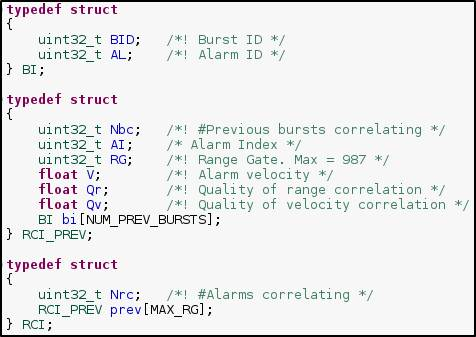
\includegraphics[width=90mm]{figures/biv_struct1}
	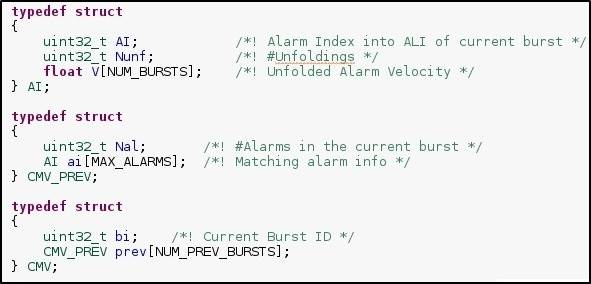
\includegraphics[width=90mm]{figures/biv_struct2}
	\caption{Structure of RCI and CMV}
	\label{fig:mm:biv_struct}
\end{figure}


\begin{figure}[h!]
	\centering
	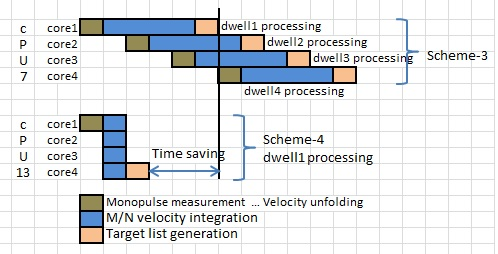
\includegraphics[width=95mm]{figures/scheme5_corr_dd}
	\caption{Comparison of Correlation Processing Schemes}
	\label{fig:mm:scheme5_corr_dd}
\end{figure}

\begin{figure}[h!]
	\centering
	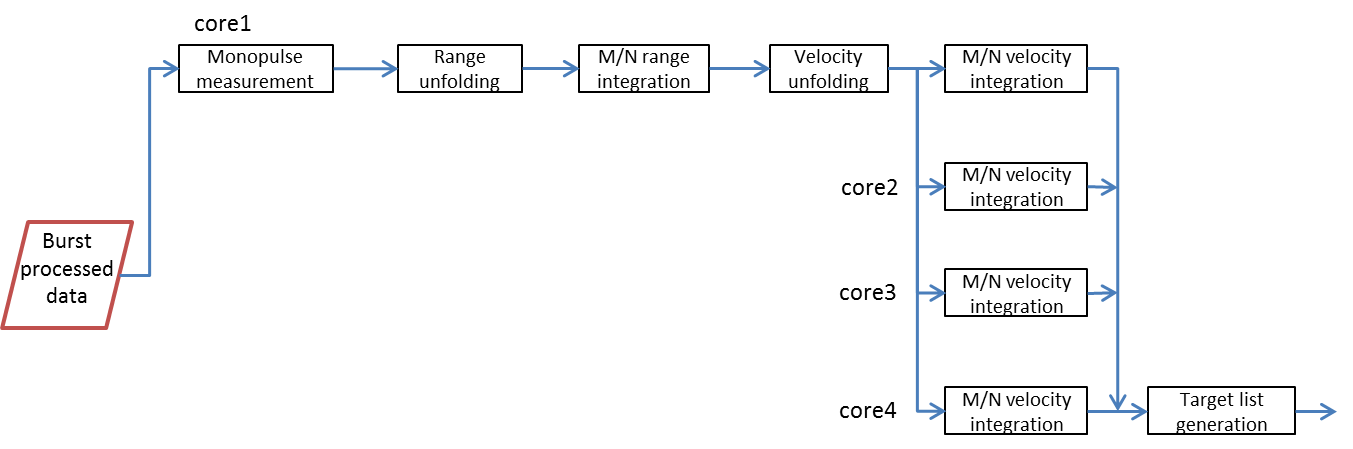
\includegraphics[width=140mm]{figures/scheme5_corr_data_path}
	\caption{Correlation Processing - Data Dependency and Mode Mapping}
	\label{fig:mm:scheme5_corr_data_path}
\end{figure}
At first, core1 receives the dwell data for correlation processing, it does Monopulse measurement, Range unfolding, M/N range integration and Velocity unfolding serially. Afterwards four threads are spawned to perform M/N velocity integration in parallel; each tread is allocated to a core. The thread completing M/N range integration last, will perform Target list generation followed by sending out the results to tracking/display processor via PSM1. 0.02ms overhead is assumed to spawn the threads and collect the results back. Resulting correlation processing time is calculated as follows. (Note: Execution time of the correlation processing steps can be seen in Figure \ref{fig:mm:scheme4_corr_calc})

\begin{align*}
\label{aa:scheme5:corr}
	Correlation \: processing \: time &= Monopulse \: measurement...Velocity \: unfolding  \\
	& \: \: + M/N \: velocity \: integration + Target \: list \: generation \\
	& \: \: + Overhead \\
	&= 4.09 + 7.93 + 0.02 + 0.02 = 12.06 \: ms \\ \stepcounter{equation}\tag{\theequation} 
\end{align*}

\subsection{CPU Load}
\label{ss:mm:scheme5:cpu_load}
Twelve CPUs are processing one burst each. Available time of a CPU is the time span between reception of two bursts to the CPU, which is 12x average burst time. As shown in Figures \ref{fig:mm:scheme5_cpu_util1} and \ref{fig:mm:scheme5_cpu_util2}, it is implied that the peak CPU utilization reaches up to 50.8\%. Look direction-2 to 4 are not shown in the figures for simplicity. Look direction-5 contributes to the worst case, as the PRF and pulse count configuration yields higher amount of data to be processed.

\begin{figure}[h!]
	\centering
	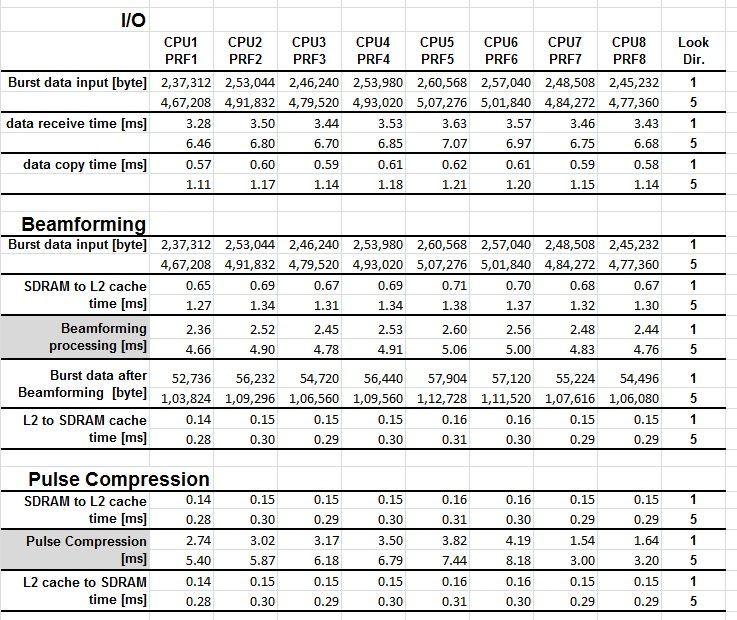
\includegraphics[width=160mm]{figures/scheme5_cpu_util1}
	\caption{Scheme-4, CPU Utilization (1/2)}
	\label{fig:mm:scheme5_cpu_util1}
\end{figure}
Nothing has changed in I/O processing and Burst data input of the Beamforming. CPU time spent on processing is explained for PRF1, look direction-1. Listed calculations illustrate one channel processing per core, as shown in the data dependency diagram \ref{fig:mm:scheme5_data_path}.

\begin{align*}
\label{aa:scheme5:equ1}
	SDRAM \: to \: L2cache &= 237,312 byte \, * \, 2.18\frac{cycle}{byte} \, * \, 1.25\frac{ns}{cycle} = 0.65 \: ms \\[0.3cm]
	Beamforming &= 1channel * 64pulses * 103 \frac{range gates}{pulse} * 287\frac{cycle}{8 element} \\[0.3cm] 
	&\qquad * 1.25\frac{ns}{cycle} = 2.36 \: ms\\[0.3cm]
	Beamformed \: data &= 1channel * 64pulses * 103 \frac{range gates}{pulse} *8\frac{byte}{sample} = 52,736 \: byte \\[0.3cm]
	L2cache \: to \: SDRAM &= 52,736 byte \, * \, 2.18\frac{cycle}{byte} \, * \, 1.25\frac{ns}{cycle} = 0.14 \: ms \\
	Pulse \: compression &= \bigg(\#channel * \#pulses (CONV128 +  \# \frac{range gates}{pulse} * RMY50)\bigg) \\
			& \quad * cycle \: time \\
			&= (1 * 64 (27300 + 103 * 68)) * 1.25ns = 2.74 \: ms \stepcounter{equation}\tag{\theequation} 
\end{align*}

\begin{figure}[h!]
	\centering
	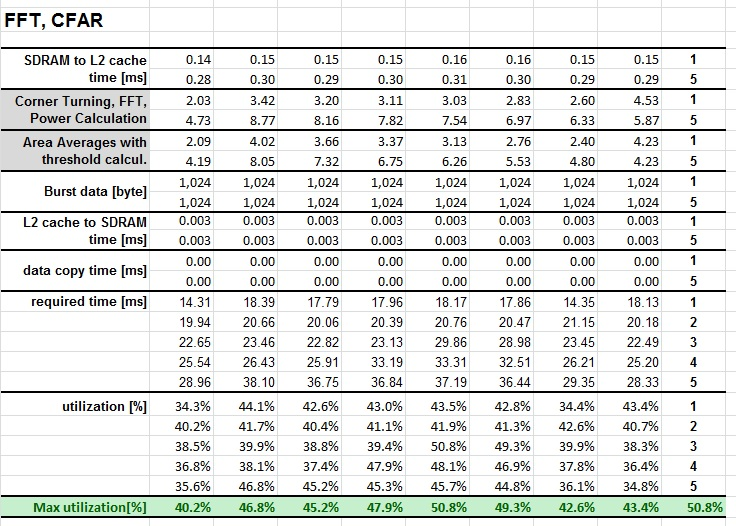
\includegraphics[width=160mm]{figures/scheme5_cpu_util2}
	\caption{Scheme-4, CPU Utilization (2/2)}
	\label{fig:mm:scheme5_cpu_util2}
\end{figure}

\begin{align*}
	FDP \: time &= \bigg(1channel * (\#pulses * \# \frac{RG}{pulse} (COT50 + RMY50) + \# \frac{RG}{pulse} * \\
		& \qquad FFT64) + 1 * (\# \frac{range gates}{pulse} * 64 * MAG256)\bigg) * cycle \, time \\[0.3cm]
		&= (1 * (64 * 103 (98 + 68) + 103 * 2550) + 1 * (103 * 64 * 41)) * 1.25ns \\
		&= \enspace 2.03 \: ms \\
		Average \: Calculation &= 1channel * 103 \frac{range gates}{pulse} * 64(FFTsize) * 51(AVG100) * 2 \\
		&=  672,384 \: cycle \\
		Thresholding &= 1channel * 103 \frac{range gates}{pulse} * 64(FFTsize) * 55(CMPR100) \\
		&= 362,560 \: cycle \\
		Detection &= 103 \frac{range gates}{pulse} * 64(FFTsize) * 97(DET100) = 639,424 \: cycle \\
		Sum \: time &= (Average \: calculation + Thresholding + Detection) * cycle \: time \\
		&= (672,384 + 362,560 + 639,424) * 1.25ns = 2.09 \: ms	\stepcounter{equation}\tag{\theequation} 
\end{align*}

Total time required to process one channel of a burst by a core is calculated as the sum of IO processing, Beamforming, Pulse compression, FFT, CFAR, Thresholding, Detection and data copy time between SDRAM to the core. CPU utilization is the ratio of processing time to the available time. Calculations for the look direction-1, CPU1 is explained here.

\begin{align*}
	Available \: time &= \#CPUs * Avg. \: burst \: time = 12 * \frac{27.84ms (dwell \: time)}{8(\#burst)} = 41.76 \: ms\\[0.3cm]
	CPU \: utilization &= \frac{processing \: time}{available \: time} = \frac{14.31}{41.76} = 34.3\% \stepcounter{equation}\tag{\theequation} 
\end{align*}

\subsubsection{Correlation Processing} 
The data processed by the CPU1...12 are grouped as dwells and sent to CPU13 and CPU14 alternatively. Correlation processing CPUs are in idle state until they receive a dwell data then performs computation for 12.06ms followed by waiting for next set of burst results from the next dwell. 0.02ms time delay between burst processing CPUs and correlation processing CPUs is assumed. Timeline diagram is illustrated in Figure \ref{fig:mm:scheme5_corr_timeline}. Utilization calculations for the look direction-1 are listed below. 

\begin{figure}[h!]
	\centering
	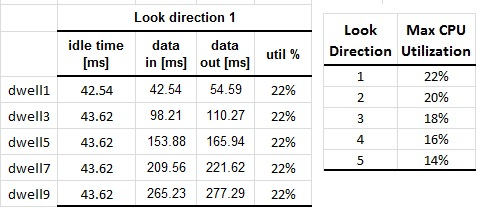
\includegraphics[]{figures/scheme5_mul_cpu_util}
	\caption{Scheme-4, Utilization of Correlation Processing CPU}
	\label{fig:mm:scheme5_mul_cpu_util}
\end{figure}

\begin{figure}[h!]
	\centering
	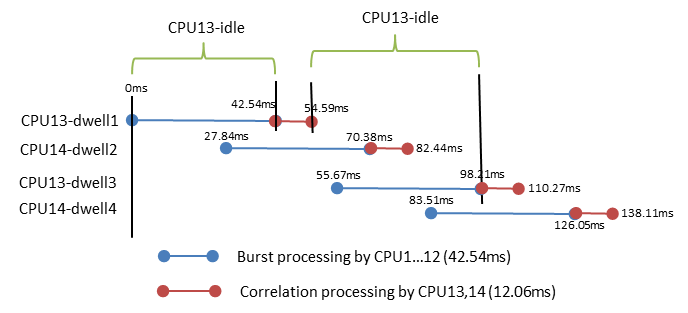
\includegraphics[]{figures/scheme5_corr_timeline}
	\caption{Look Direction-1, Utilization of the Correlation Processing CPU}
	\label{fig:mm:scheme5_corr_timeline}
\end{figure}

\begin{align*}
	Utilization \: at \: dwell1 &= \frac{processing \: time}{processing \: time + waiting \: time } = \frac{12.06}{12.06 + 42.54} = 22\% \\[0.4cm]
	Next \: dwell \: time &= Dwell3 \: input \: at \: burst \: processing + Burst \: processing \: time \\
	&= 2 * 27.84 + 42.54 = 98.2 \: ms\\
	Idle \: time &= Next \: dwell \: in - Last \: dwell \: out \\
	&= 98.2 - (12.06 + 42.54) = 43.6 \: ms \\
	Utilization \: at \: dwell3 &=  \frac{12.06}{12.06 + 43.6} = 22\%  \stepcounter{equation}\tag{\theequation}
\end{align*}
From the Figure \ref{fig:mm:scheme5_mul_cpu_util}, peak utilization of the correlation processing CPU reaches upto 22\% when using two CPUs. 

\subsection{Processing Latency}
\label{ss:mm:scheme5:latency}
Processing latency between 54.79ms and 88.17ms is achieved depending on the look direction, which is the time required for burst processing and correlation processing. Maximum dwell latency is 1.97x dwell time contributed by the look direction-1. The processing latencies of the look direction-1...5 are listed below. 

\begin{table}[h!]
	\centering
	\begin{tabular}{|c|l|l|l|} 
	 \hline
	 \textbf{Look direction} & \textbf{Dwell time[ms]} & \textbf{Latency[ms]} & \textbf{\#Dwell latency} \\
	 \hline
	 1 & 27.84 & 54.79 & 1.97 \\ \hline
	 2 & 33.07 & 61.43 & 1.86 \\ \hline
	 3 & 39.17 & 69.10 & 1.76 \\ \hline
	 4 & 46.20 & 77.98 & 1.69 \\ \hline
	 5 & 54.26 & 88.17 & 1.62 \\ \hline
	\end{tabular}
	\caption{Scheme-4, Processing Latency}
	\label{tbl:mm:scheme5_latency}
\end{table}

\subsection{Memory Utilization}
\label{ss:mm:scheme5:mem_util}
From the \verb|mem_util.sh| script, it is measured that the Radar application is consuming only 0.5\% of the available 879MiB memory. Memory requirement is reduced since, one CPU is working on one burst data, whereas in Scheme-3, one CPU gets 4 burst data. Memory utilization footprint of the Radar application is shown in Figure \ref{fig:mm:scheme4_mem_util}. Though the memory requirement is reduced by a factor of 4, memory utilization of the Radar application is not reduced by the same figure. Since, the Radar application has SQLite library, FFTW library, spawning threads and other processing steps are required to run the application, they consume certain amount of memory regardless of the input data set.

\begin{figure}[h!]
	\centering
	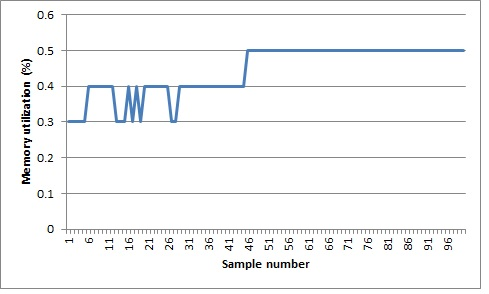
\includegraphics[width=100mm]{figures/scheme5_mem_util}
	\caption{Scheme-4, Memory Utilization Footprint}
	\label{fig:mm:scheme5_mem_util}
\end{figure}


\subsection{Memory Transfer Bandwidth}
\label{ss:mm:scheme5:bw_util}
Memory footprint is reduced compared to the Scheme-3, leading to a smaller amount of operating data set per core. Private L1 cache and shared L2 cache can hold large portion of the operating data set, reducing memory transfer between SDRAM to core and so reducing memory transfer bandwidth. The lowest recorded memory transfer bandwidth by running the STREAM benchmark as a background task is listed in Table \ref{tbl:mm:scheme5_mem_bw}. Peak memory transfer bandwidth of the Radar application is measured as 30.3\% of the available 1048MiB/s.

\begin{table}[h!]
	\centering
	\begin{tabular}{|l|l|l|l|l|} 
	 \hline
	 \textbf{Function} & \textbf{Best Rate [MB/s]} & \textbf{Avg time[s]} & \textbf{Min time[s]} & \textbf{Max time[s]} \\
	 \hline
	 Copy & 729.9 & 0.253547 & 0.219210 & 0.300818\\ \hline
	\end{tabular}
	\caption{Recorded Memory Transfer Bandwidth of the STREAM Benchmark Running as Background Task}
	\label{tbl:mm:scheme5_mem_bw}
\end{table}

\begin{align*}
\label{aa:scheme4:mem_bw}
	Peak \: BW \: of \: the \: Radar \: application &= Idle \: BW - Lowest \: recorded \: BW \\
	&= 1048 - 729.9 =  318.1 \: MiB/s \\
	&= \frac{318.1}{1048} = 30.3 \% \stepcounter{equation}\tag{\theequation} 
\end{align*}

\subsection{Summary}
\label{ss:mm:scheme5:summary}

Processing latency of 1.92x dwell time and peak CPU utilization of 50.8\% are healthy values for Air to Air Mode Radar processor. It has remaining 49\% of the CPU utilization to accommodate future development. In fact, 8 CPUs are sufficient to give same processing latency. More CPUs are used to improve the utilization. Figure \ref{fig:mm:scheme5_summary} shows the relationship between number of CPUs used and their utilization without affecting the latency values. Any combination of the CPU sets can be chosen to achieve desired CPU load. Selecting 10 CPUs for burst processing and 1 CPU for correlation processing will have peak CPU utilization of 61\% and 1.92x dwell latency, leaving rest of the 13 CPUs for A/G mode processing in an IMA processor architecture. A comparison of  Scheme-1, Acceptable values and Scheme-4 is listed in Table \ref{tbl:mm:scheme5_comparison}.

\begin{figure}[h!]
	\centering
	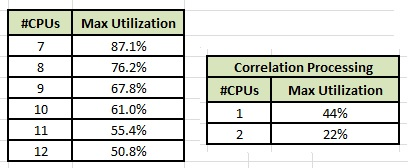
\includegraphics[width=90mm]{figures/scheme5_summary}
	\caption{Scheme-4, Relationship Between Number of CPUs and Utilization}
	\label{fig:mm:scheme5_summary}
\end{figure}

\begin{table}[h!]
	\centering
	\begin{tabular}{|l|l|l|l|} 
	 \hline
	 \textbf{Parameter} & \textbf{Scheme-1} & \textbf{Acceptable Values} & \textbf{Scheme-4}\\
	 \hline
	 Dwell latency &  14.96 & 2 & 1.97 \\ \hline
	 CPU load & 75.5\% & \textless 50\% & 50.8\% \\ \hline
	 Memory Utilization & 7\% & \textless 50\%  & 0.5\% \\ \hline
	 Memory transfer bandwidth & NA & \textless 50\% & 30\%  \\ \hline
	\end{tabular}
	\caption{Comparison of Scheme-1 vs Acceptable Values vs Scheme-4}
	\label{tbl:mm:scheme5_comparison}
\end{table}

\section{Overview}
The Existing Analysis has been observed to spot the latency contributors, bottlenecks and data dependencies. Upsides and downsides are evaluated to bring up a best mode mapping scheme. Examined information have supported in design decisions of the mode mapping. Two new schemes are proposed to reduce the processing latency and they are validated via implementation. \vspace*{0.2cm}

Scheme-3 makes use of the fact that, the bursts in a dwell can be processed independently until the Thresholding and Detection stage. This phenomenon skips waiting time in Beamforming, Pulse compression, FFT, CFAR, Thresholding and Detection stage. This can be called as coarse grained parallelism. A dedicated processor is assigned for Correlation processing, without changing the execution method. Final outcome of the Scheme-3 is 4x dwell latency with 66\% CPU utilization. \vspace*{0.2cm}

Every burst data has large amount of fine grained parallelism. Four channel processing of a burst is done independently in Scheme-4, saving the waiting time for the other channel processing.  Correlation processing poses a bottleneck as the serial execution requires 1.5x dwell time. Further, it is also parallelised and executed in dedicated CPUs. Deemed 2x processing latency is achieved along with 50.8\% CPU utilization, provided 13 CPUs are performing computation. From the Table \ref{tbl:mm:scheme5_comparison} data, speedup of the Scheme-4 compared to the best scheme(Scheme-1) in the Existing Analysis is drawn as follows. \\

\begin{figure}[h!]
\centering
	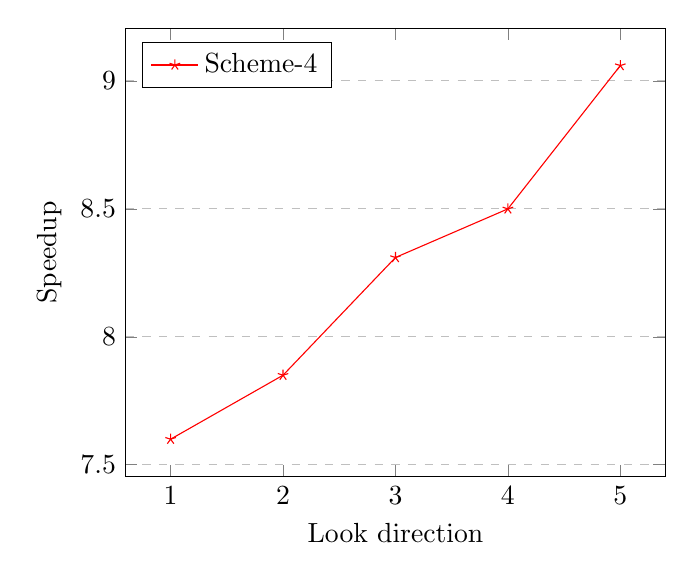
\begin{tikzpicture}
		\begin{axis}[
			xlabel={Look direction},
			ylabel={Speedup},
			legend pos=north west,
			ymajorgrids=true,
			grid style=dashed,
		]
		\addplot[color=red, mark=star,]
			coordinates {
				(1, 7.6) (2, 7.85) (3, 8.31) (4, 8.50) (5, 9.06)
			};
		\legend{Scheme-4}
	\end{axis}
\end{tikzpicture}
\caption{Speedup, Scheme-4 vs Scheme-1}
\label{mm:scheme5_speedup}
\end{figure}

The best results of the Existing Analysis are 75.5\% peak CPU utilization and 15x dwell latency, provided 12 CPUs are executing the Radar processing algorithm. For the same utilization value, Scheme-4 needs only 9 CPU resources and delivers acceptable latency of 2x dwell time.

\clearpage
\section{Verification of Results}
\label{mm:sec:verification_of_results}
To verify the correctness of the Scheme-3 and Scheme-4 implementations, the results of the 4-core implementations are cross checked against the single core implementation. Both the results are matching, assuring that the application is producing consistent results in single-threaded and multi-threaded environment.